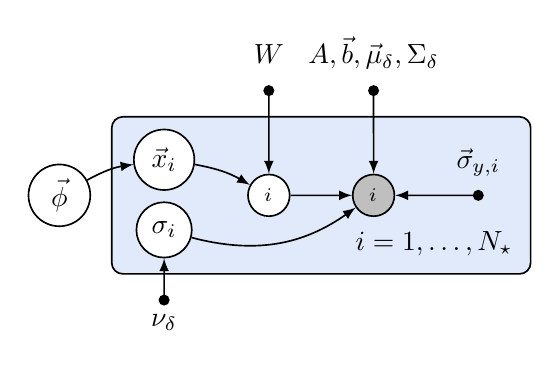
\begin{tikzpicture}[scale=1.33, line width=0.6pt, every node/.style={circle, draw, fill=white}, >=latex]

    \draw[fill=CornflowerBlue!20, rounded corners] (0.5, 0.25) rectangle (4.5, 1.75);
    \node[rectangle, draw=none, fill=none, above left=3pt, align=right] at (4.5, 0.25) {$i = 1, \dots, N_\star$};
    \node (hyper) at (0, 1) {$\vec\phi$};
    \node (inputs) at (1, 1.34) {$\vec x_i$} edge [<-, bend right=10] (hyper);
    \node (error) at (1, 0.67) {$\sigma_i$};
    \node (outputs) at (2, 1) {$\pred_i$} edge [<-, bend right=10] (inputs);
    \node [fill=black!25] (observables) at (3, 1) {$\obs_i$} edge [<-] (outputs) edge [<-,bend left=25] (error);

    \fill (1, 0) circle (1.5pt) edge [->] (error) node[below=3pt, fill=none,draw=none, rectangle, text height=3pt] {$\nu_\delta$};
    \fill (2, 2) circle (1.5pt) edge [->] (outputs) node[above=3pt, fill=none,draw=none, rectangle, text depth=3pt] {$\mat W$};
    \fill (3, 2) circle (1.5pt) edge [->] (observables) node[above=3pt, fill=none,draw=none, rectangle, text depth=3pt] {$\mat A, \vec b, \vec\mu_\delta, \mat\Sigma_\delta$};
    \fill (4, 1) circle (1.5pt) edge [->] (observables) node[above=3pt, fill=none,draw=none, rectangle, text depth=3pt] {$\vec\sigma_{y, i}$};

\end{tikzpicture}

